\documentclass[conference]{IEEEtran}
% correct bad hyphenation here
\hyphenation{op-tical net-works semi-conduc-tor}

\usepackage[utf8]{inputenc} % Document UTF8
\usepackage[francais]{babel} % Le document est en francais
\usepackage[T1]{fontenc} % Suppression d'un warning
\usepackage{graphicx} % Insertion d'images
\usepackage{amsmath} % Package mathématiques
\usepackage{tikz} % Diagramme camembert
\usepackage{colortbl} % Couleur dans les tableaux

\begin{document}
%
% paper title
% can use linebreaks \\ within to get better formatting as desired
\title{Rapport : Analyse individuelle d'un site web}

% author names and affiliations
% use a multiple column layout for up to three different
% affiliations
\author{\IEEEauthorblockN{Florian Thuin}
\IEEEauthorblockA{06561100\\
SINF13BA}}

% make the title area
\maketitle


\begin{abstract}
%\boldmath
Ce rapport décrit l'analyse du site 7sur7.be dans le cadre du cours LINGI1341 - Réseaux informatiques.
\end{abstract}

\IEEEpeerreviewmaketitle



\section{Introduction}

7sur7 est un site belge d'informations et de sports. De par sa nature, ce site dispose d'un contenu divers et changeant (photos, textes, publicités, plugins sociaux,...), au vu de la quantité de données partagée lors d'une connexion à ce site, il est impossible d'en traiter l'entièreté, ce rapport n'est donc qu'un résumé de certaines interactions jugées intéressantes entre moi (le client) et les différents serveurs de données.
 
\hfill 16 décembre 2014

\section{Les requêtes au résolveur de noms de domaines}

La page d'accueil du site entraînant à elle seule 150 requêtes DNS, la majorité d'entre elles ne seront pas analysées dans ce rapport.

\subsection{Les requêtes et réponses majoritaires}

Pour chaque nom de domaine auquel la page me demande d'accéder pour récupérer de l'information, une requête de type IPv4 et une autre de type IPv6 est envoyée. En analysant les réponses à ces requêtes, je me suis rapidement rendu compte que la majorité des noms de domaine accédés n'ont pas un serveur qui leur est entièrement dédié et renvoie donc un CNAME. Ces CNAME sont en grande partie des serveurs EdgeSuite, un réseau de serveurs fournisseurs de contenus (CDN) de la société Akamai Technologies[1]. Le passage par ses serveurs se fait pour des raisons économiques, de performances et de pannes[2]. Environ 7\% des réponses ont retourné une adresse IPv6, ce qui correspond plus ou moins à la représentation actuelle du trafic[3], les autres serveurs sont encore limités à l'IPv4.

\subsection{Les requêtes répétées}

Pour certains serveurs web, plusieurs requêtes DNS sont envoyées avec la même ID depuis le même port pour le même nom de domaine. Les serveurs DNS lui répondent comme prévu, mais toutes les réponses qui suivent la première sont refusées même si elles contiennent un contenu différent et un message est transmis en ICMP au serveur DNS lui signalant Destination Unreachable (Port Unreachable). Je n'ai pas de pistes d'explication sur l'intérêt de ces requêtes multiples à moins d'une milliseconde d'intervalle et encore moins avec la même ID puisque pour éviter le DNS spoofing, la première réponse gagne toujours[4]. Pour mieux faire, je ne devrais consulter qu'un seul serveur DNS.

\begin{tabular}{|l|l|l|}
 \hline
 \rowcolor{gray!60} Time & IPsrc & IPdst \\
 \hline
 \rowcolor{cyan} 8.164024 & 130.104.157.67 & 130.104.1.2 \\
 \multicolumn{3}{|p{8cm}|}{Standard query 0x6785  A gabe.hit.gemius.pl} \\
 \hline
 \rowcolor{cyan} 8.164039 & 130.104.157.67 & 130.104.1.1 \\
 \multicolumn{3}{|p{8cm}|}{Standard query 0x6785  A gabe.hit.gemius.pl} \\
 \hline
 \rowcolor{cyan} 8.164044 & 130.104.157.67 & 130.104.254.1 \\
 \multicolumn{3}{|p{8cm}|}{Standard query 0x6785  A gabe.hit.gemius.pl} \\
 \hline
  \hline
 \rowcolor{cyan} 8.275129000 & 130.104.1.1 & 130.104.157.67 \\
  \multicolumn{3}{|p{8cm}|}{Standard query response 0x6785  A 213.189.48.245 A 213.189.48.246 A 213.189.48.247 A 213.189.48.205 A 213.189.48.206 A 213.189.48.207 A 213.189.48.208 A 213.189.48.242 A 213.189.48.243 A 213.189.48.244} \\
  \hline
 \rowcolor{red!70} 8.275384000 & 130.104.1.2 & 130.104.157.67 \\
  \multicolumn{3}{|p{8cm}|}{Standard query response 0x6785  A 213.189.48.205 A 213.189.48.206 A 213.189.48.207 A 213.189.48.208 A 213.189.48.242 A 213.189.48.243 A 213.189.48.244 A 213.189.48.245 A 213.189.48.246 A 213.189.48.247} \\
  \hline
 \rowcolor{black!65} 8.275424000 & 130.104.157.67 & 130.104.1.2 \\
  \multicolumn{3}{|p{8cm}|}{Destination unreachable (Port unreachable)} \\
  \hline
 \rowcolor{red!70} 8.279695000 & 130.104.254.1 & 130.104.157.67 \\
  \multicolumn{3}{|p{8cm}|}{Standard query response 0x6785  A 213.189.48.206 A 213.189.48.207 A 213.189.48.208 A 213.189.48.242 A 213.189.48.243 A 213.189.48.244 A 213.189.48.245 A 213.189.48.246 A 213.189.48.247 A 213.189.48.205} \\
  \hline
 \rowcolor{black!65} 8.279730000 & 130.104.157.67 & 130.104.254.1 \\
  \multicolumn{3}{|p{8cm}|}{Destination unreachable (Port unreachable)} \\
  \hline
\end{tabular}


\subsection{Les domaines liés directement au site}

www.7sur7.be, static0.7sur7.be, static1.7sur7.be, static2.7sur7.be, static3.7sur7.be sont les seuls noms de serveurs qui délivrent réellement du contenu relatif à la description du site web. Ceux-ci délivrent la plus grosse partie des données pouvant suffire à un affichage basique du site et sont liés à des serveurs CDN d'Akamai (tous sous le CNAME dpp-cdn.be.edgesuite.net). 

\subsection{Les autres domaines}

Dans les autres noms de serveurs accédés, il y a des réseaux sociaux (Facebook, Twitter), des \og{} partenaires \fg{} commerciaux (L'Echo, HetLaastNieuws, PersGroep), des publicitaires (serving-sys.com de EyeBlaster, doubleclick.net;googlesyndication.com de Google) et des analyseurs de traffic (newrelic.com, adhese.com, chartbeat.net, gemius.pl, google-analytics.com).

\section{Les requêtes HTTP}

Toutes les requêtes HTTP sont en version 1.1, autrement dit il y a la possibilité de garder une connexion TCP pour accéder à plus d'un URI. Les ressources accédées sont (par ordre décroissant) le JPG, JavaScript, PNG, HTML, GIF, CSS, Flash, WOFF. Sans mise en cache, les données vont jusqu'à 7Mo (selon les jours) de données compressées (gzip, deflate). 

\begin{tabular}{cc}
 \begin{tikzpicture}[scale=0.35]
 \foreach \a/\b/\p/\i/\c in
  {
    0/3.6/1/red/Flash, 3.6/28.8/7/blue/CSS,
    28.8/57.6/8/green/HTML, 57.6/158.4/28/yellow/Javascript,
    158.4/360/56/purple/Image
  }
  {
    \draw[fill=\i!65]
    (0,0) -- (\a:4.5) arc (\a:\b:4.5) -- cycle;
    \draw ({(\a+\b)/2}:4) node {\p\%};
    \draw ({(\a+\b)/2}:5.6) node {\c};
  }
\end{tikzpicture} &
\begin{tikzpicture}[scale=0.35]
 \foreach \a/\b/\p/\i/\c in
  {
    0/7.2/2/red/Flash, 7.2/18.0/3/blue/CSS,
    18.0/43.2/7/green/HTML, 43.2/190.8/41/yellow/Javascript,
    190.8/360/46/purple/Image
  }
  {
    \draw[fill=\i!65]
    (0,0) -- (\a:4.5) arc (\a:\b:4.5) -- cycle;
    \draw ({(\a+\b)/2}:4) node {\p\%};
    \draw ({(\a+\b)/2}:5.6) node {\c};
  }
\end{tikzpicture} \\
  \emph{Répartition sans cache} & \emph{Répartition avec cache} \\
\end{tabular}


Sur la page d'accueil, en dehors du script de connexion au site web qui est chargé en HTTPS, toutes les ressources sont chargés en HTTP. D'autres requêtes sont faites en HTTPS mais elle concerne les trackers (Newrelic \& Chartbeat).

Je remarque qu'il y a dans les en-têtes HTTP des informations qui sont pour moi redondantes puisque plusieurs options agissent de manière similaire. Cela est peut-être dû à mon manque de connaissance de ce domaine, cependant beaucoup de mes réponses utilisent le header Cache-Control avec les options max-age=0, no-cache, no-store, must-revalidate, le header Pragma avec l'option no-cache et une date d'expiration datée avant les années 2000 (et max-age outrepasse Expires). Le seul intérêt que j'y vois est de s'assurer qu'aucun client quel qu'il soit ne stocke l'information envoyée, c'est utile pour des statistiques d'utilisation du site. Et au contraire, certaines réponses demandent à être stockées en cache durant 1 mois. 

\subsection{Les headers utilisés}

\begin{description}
 \item[Accept : ] ce header permet de spécifier le type de ressource MIME que l'on souhaite. Le navigateur peut en spécifier plusieurs et leur donner des préférences en utilisant une q-valeur.
 \item[Content-Type : ] header permettant de dire le type de ressource renvoyée, pour les sites optimisés le même que celui mis dans Accept avec la préférence la plus grande.
 \item[Accept-Encoding : ] ce header permet de spécifier l'encodage, Firefox utilise sur ce site principalement gzip et deflate pour recevoir des données compressées, ce qui permet de faire des économies en bande passante.
 \item[Accept-Language : ] ce header permet de spécifier une langue de préférence selon les préférences du navigateur avec des préferences en utilisant une q-valeur.
 \item[Date : ] la date de la réponse.
 \item[Expires : ] ce header permet de spécifier la date d'expiration du document MIME pour signifier qu'il faut le recharger après cette date.
 \item[If-Modified-Since : ] ce header permet de spécifier la date de la mise en cache pour ne pas recharger des données encore à jour.
 \item[Etag : ] Un hash qui identifie la version d'une ressource.
 \item[If-None-Match : ] ce header fonctionne comme If-Modified-Since mais avec un Etag au lieu d'une date.
 \item[Last-Modified : ] ce header permet de signifier la dernière date de modification. Si cette date est ultérieure à If-Modified-Since, le contenu sera mis à jour, sinon la réponse aura un code 304 - Not modified.
 \item[Cache-Control : ] ce header permet de spécifier des paramètres de cache. Le max-age définit le temps en secondes maximum de rétention dans la cache. Il est moins prioritaire que le header Expires.
 \item[Cookie : ] ce header permet au client d'envoyer le cookie qu'il contient pour l'identifier.
 \item[User-Agent : ] permet au serveur de connaître le client et sa version, le système d'exploitation et sa version, ce qui peut lui permettre d'afficher du contenu optimisé pour le client.
 \item[Connection : ] indique le type de connexion que le client ou le serveur souhaite (keep-alive ou close).
 \item[Server : ] le type du serveur qui a répondu.
 \item[Content-Length : ] la longueur du contenu en bytes.
 \item[Referer : ] l'adresse visitée avant d'être dirigée sur le contenu. Utile pour connaître le comportement de l'utilisateur.
 \item[Content-Location : ] le chemin réel vers le contenu demandé.
 \item[X-Requested-With : ] permet d'envoyer une valeur pour identifier une requête Ajax. (non-standard)
 \item[X-Powered-By : ] indique la technologie utilisée pour la web application, e.g; JSP/2.2. 
 \item[X-UA-Compatible : ] recommande le client préféré pour afficher le contenu, e.g. IE=Edge. (non-standard) 
 \item[uniqueRequestId : ] pas d'explication claire, envoyé lorsque le serveur utilise JSP, certaines sources disent que c'est utilisé pour du débogage, 
\end{description}

\subsection{Requête et réponse non-standard}

Voici quelques requêtes qui ne sont pas explicables par la matière vue en cours.

GET https://caps.7sur7.be/service/ssologin/ssoconnect.js
\begin{tabular}{|r|p{5cm}|}
  \hline
  Réponse & \\
  \hline
  Cache-Control & max-age=2592000, no-transform,public,max-age=300,s-maxage=900 \\
  \hline
\end{tabular}

Ce header de réponse m'a étonné puisqu'il signifie deux fois le paramètre max-age et une fois le paramètre s-maxage. s-maxage permet de définir un temps pour le shared-cache (qui prévaut sur une directive max-age) et max-age pour le private-cache[9], cependant je ne vois pas l'intérêt d'avoir deux paramètres max-age puisqu'un des deux doit être prioritaire sur l'autre, cela peut peut-être provoquer des comportements différents. \\
\\

GET http://www.7sur7.be/static/nmc/nmc/head/autodeploy .css?20140811.3 \\

\begin{tabular}{|r|p{5cm}|}
  \hline
  Réponse & \\
  \hline
  X-N & S \\
  \hline
\end{tabular}

Après de nombreuses recherches, cet header semble typique d'Akamai mais l'utilité réelle n'est pas définie. Certains firewalls conseillent de bloquer les réponses contenant ce type de header puisqu'on ne peut pas trouver de documentation sur leur utilisation[10]. Cependant, si c'était le cas mon site perdrait un CSS de 1615 bytes et le style du site serait probablement mis à mal.

GET /partner/index?module=combo\&style=vertical\&
locale=fr\_BE\&utmparams\%5Butm\_source\%5D=7sur7\&
utmparams\%5Butm\_campaign\%5D=landelijk\&utmparams\%
5Butm\_medium\%5D=partnermodule\&listingparams\%
5BminPrice\%5D=2999\&listingparams\%5Blimit\%5D=2\&
listingparams\%5Bsort\%5D=random\&listingparams\%5BminPhotos\%
5D=3\&listingparams\%5BbuildYearFrom\%5D=2008 HTTP/1.1

\begin{tabular}{|r|p{5cm}|}
  \hline
  Requête & \\
  \hline
  Accept & */* \\
  Accept-Encoding & gzip, deflate \\
  Accept-Language & fr, fr-fr;q=0.8,en-us;q=0.5,en;q=0.3 \\
  Connection & keep-alive \\
  Host & fr.autotrack.be \\
  Referer & http://www.7sur7.be/ \\
  User-Agent & Mozilla/5.0 (X11; Ubuntu; Linux x86\_64; rv:34.0) Gecko/20100101 Firefox/34.0 \\
  \hline
  Réponse & \\
  \hline
  Cache-Control & no-cache, no-store, must-revalidate \\
  Connection & keep-alive \\
  Content-Encoding & gzip \\
  Content-Length & 3666 \\
  Content-Type & text/javascript;charset=utf-8 \\
  Date & Sat, 13 Dec 2014 10:49:37 GMT \\
  Expires & Sat, 13 Dec 2014 10:49:37 GMT \\
  P3P & policyref=/w3c/p3p.xml, CP="NOI DSP COR NID CUR ADM DEV OUR BUS" \\
  Pragma & no-cache \\
  Server & Apache/2.2.3 (Red Hat) \\
  Vary & Accept-Encoding \\
  X-Varnish & 82859191 \\
  \hline
\end{tabular}

La requête correspond aux normes HTTP, mais la réponse est assez particulière. Il y a une redondance des informations, si la date d'expiration vaut la date de réception, elle ne devrait pas être reprise dans le cache, donc l'option no-cache est redondante, no-store s'y ajoute, ce qui fait que le client devrait forcément se reconnecter au serveur pour récupérer la donnée la prochaine fois, mais malgré tout il y a un must-revalidate qui en ajoute une couche. Cette requête utilise X-Varnish, qui est selon le site de Varnish une ID utile pour déboguer[5]. Varnish définit d'autres headers qui sont vus dans d'autres requêtes sur www.7sur7.be comme X-Cacheable et X-Varnish-Cache pour définir des propriétés spéciales sur ses objets en cache.  Elle utilise également une technique pour informer l'utilisateur sur l'utilisation des informations récoltées mais cette technologie n'est plus mise à jour depuis 2006 [6]. Cependant, GoogleAdServices informe également les utilisateurs de cette manière. 

Les requêtes à GoogleSyndication (serveur pub de Google) donnent aussi lieu à certains headers non-attendus :
\begin{tabular}{|r|p{5cm}|}
  \hline
  Requête & \\
  \hline
  Accept & image/png,image/*;q=0.8,*/*;q=0.5 \\
  Accept-Encoding & gzip, deflate \\
  Accept-Language & fr, fr-fr;q=0.8,en-us;q=0.5,en;q=0.3 \\
  Connection & keep-alive \\
  Host & pagead2.googlesyndication.com \\
  Referer & http://www.7sur7.be/ \\
  User-Agent & Mozilla/5.0 (X11; Ubuntu; Linux x86\_64; rv:34.0) Gecko/20100101 Firefox/34.0 \\
  \hline
  Réponse & \\
  \hline
  Alternate-Protocol & 80:quic,p=0.02 \\
  Cache-Control & no-cache, no-store, must-revalidate \\
  Content-Length & 0 \\
  Content-Type & text/html; charset=UTF-8 \\
  Date & Sat, 13 Dec 2014 10:49:37 GMT \\
  Expires & Fri, 01 Jan 1990 00:00:00 GMT \\
  P3P & policyref="http://www.googlead services.com/pagead/p3p.xml", CP="NOI DEV PSA PSD IVA IVD OTP OUR OTR IND OTC" \\
  Pragma & no-cache \\
  Server & cafe \\
  X-XSS-Protection & 1; mode=block \\
  x-content-type-options & nosniff \\
  \hline
\end{tabular}

Google y définit un protocole alternatif QUIC (Quick UDP Internet Connections) qui est un protocole réseau expérimental de la couche transport. C'est une combinaison entre UDP pour la rapidité et TLS pour chiffrer le transfert. Le but est de contourner les limitations de TCP et d'arriver à un RTT de 0, particulièrement pour les terminaux mobiles[7]. Le header X-XSS-Protection permet de spécifier un filtre anti-\og{} Cross-site Scripting\fg{}, autrement dit éviter des attaques par injection JavaScript par un client qui pourrait modifier le comportement attendu du serveur web. Le header X-Content-Type-Options qui s'utilise toujours avec l'option nosniff permet d'interdire le \og{} Content sniffing \fg{}, autrement dit l'utilisation par un navigateur d'un algorithme pour essayer de deviner le Content-Type du document reçu. Cet algorithme qui fonctionne comme la commande File de Linux (qui indique le type d'un fichier) est vulnérable aux attaques et parmi les navigateurs les plus utilisés, il n'y a plus qu'Internet Explorer qui l'utilise encore[8]. Dans d'autres requêtes sur les publicités de Google, on peut aussi s'apercevoir que Google a créé des headers qui lui sont propres comme Google-Creative-Id et Google-LineItem-Id pour identifier ses publicités avec l'outil DoubleClick For Publishers.

\begin{tabular}{|r|p{5.1cm}|}
  \hline
  Réponse & \\
  \hline
  X-FB-Debug & zndQPYjiQVYb8tPcPxXMPMoED
  2aLW/qGdAtvJqzzJqBCTXNGp+dK
  KxCk7sIDTwPRnwJpLyqxd55lAyG
  YoDoTfw== \\
  \hline
\end{tabular}

On peut également s'apercevoir que Google ou Akamai ne sont pas les seuls à utiliser des headers particuliers puisque Facebook transmet également des informations de débogage. Facebook utilise aussi un header Content-Security-Policy qui permet de réduire l'affichage du contenu envoyé à certains sites[11].

En conclusion, on peut rencontrer une multitude de headers HTTP qui sont des extensions et qui sont créés par certaines entreprises selon leur besoin, mais n'étant malheureusement pas un professionnel et ne disposant que de quelques pages, je ne peux pas discuter sur chacun, c'est pourquoi je n'expliquerai pas d'autres headers (X-Host, Content-Security-Policy,...). 

\section{Connexions TCP}

Sur la page d'acccueil, pour récupérer toute l'information mon serveur ouvre environ 125 connexions TCP. Ce nombre peut paraître grand, puisqu'il est dit dans la section sur les requêtes DNS qu'il y a environ 150 requêtes dont 75 correspondent à de l'IPv4 qui est réellement utilisée pour se connecter. Une première explication est que malgré l'utilisation de HTTP/1.1, certains serveurs ne souhaitent pas entretenir une connexion keep-alive et renvoient close. C'est le cas environ 5 fois, donc ça n'explique pas entièrement ce nombre élevé de connexions.

Une deuxième explication est que certaines connexions s'ouvrent de manière inutile. Exemple : Le three-way handshake standard entre moi et le serveur. 2 secondes plus tard, le serveur m'envoie un RST sans qu'aucune information n'ait été partagée. Cet échange est avec un serveur de Gemius.

\begin{tabular}{|l|p{5cm}|}
 \hline
 ipSrc:port & 130.104.157.67:57237 \\
 ipDst:port & 213.189.48.245:80 \\
 \hline
 Time : & Info : \\
 8.298685 & [SYN] Seq=0 Win=29200 Len=0 MSS=1460 SACK\_PERM=1 TSval=173199 TSecr=0 WS=128 \\
 8.400664 & [SYN; ACK] Seq=0 Ack=1 Win=65535 Len=0 MSS=1460 SACK\_PERM=1 \\
 8.400726 & [ACK] Seq=1 Ack=1 Win=29200 Len=0 \\
 10.880089 & [RST; ACK] Seq=1 Ack=1 Win=65535 Len=0 \\
 \hline
\end{tabular}

Une troisième explication et certainement la plus importante est qu'il est commun pour les applications sur le web filaire d'ouvrir une connexion TCP par type de contenu qui est partagé par un nom de domaine. Cette technique peut poser des problèmes pour de la navigation mobile et les performances du site peuvent décroître[12].

Une quatrième explication est que certains contenus se rechargent après un certain temps (par exemple toutes les 5 secondes) et dans mon cas, la connexion se ferme puis se réouvre à chaque fois, parfois pour partager des ressources très faible et inutile à l'utilisateur (typiquement, les trackers avec des GIF 1x1).

La limite de 6 connexions simultanées n'est jamais atteinte sur Firefox34 et cela peut s'expliquer par le fait que le contenu est séparé sur 5 serveurs (voir Section II, C), ce qui lui offre théoriquement 30 connexions TCP simultanées.

Toutes mes connexions TCP acceptent à la création les acquittements sélectifs. le scaling factor de la taille de la window est soit de 32 (window scale = 5), soit de 128 (window scale = 7). Je n'ai pas compris l'intérêt des Timestamps, en dehors de partager le temps propre au serveur et au client en millisecondes et donc connaître la séquence des actions (ces timestamps étant observés grâce à Wireshark qui s'occupe de mettre de l'ordre lui-même et de calculer le RTT, c'est peut-être la raison pour laquelle je n'en vois pas l'intérêt puisque je ne dois plus rien en faire). Il n'y a aucune notification explicite sur la congestion window. Les discussions sur le contenu se faisant avec Akamai, on sait que la congestion window initiale est de 15, pour les publicités Google, la congestion window initiale est de 10[13].

Ce graphe montre le traffic total en bytes (en noir) et le traffic lié à mon site web en bytes (en rouge). On se rend compte que le début du chargement est lié au contenu de mon site web et que la dernière seconde de chargement est entièrement dédiée à des contenus annexes (publicités). La volatilité s'explique par le fait que c'est en Wi-Fi.

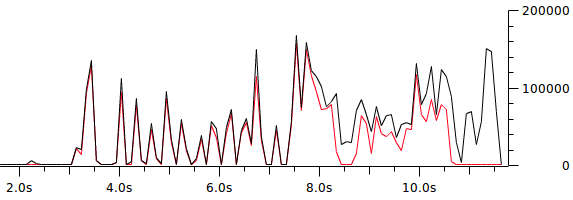
\includegraphics[scale=0.4]{tcp.png}

\section{Autres}

Ayant fait un programme de récupération des données à partir de Wireshark, j'ai également pu observer d'autres communications bizarres qui ne sont pas directement reliées à ce projet dans mes analyses. 

En faisant une capture en WiFi à partir de l'UCL, 

\begin{tabular}{|l|l|}
 \hline
 ipSrc:port & 60.173.9.36:6000 \\
 ipDst:port & 130.104.157.67:9064 (mon ip) \\
 Reçu & [SYN] Seq=0 Win=16384 Len=0 \\
 Envoyé & [RST; ACK] Seq=1 Ack=1 Win=0 Len=0 \\
 \hline
\end{tabular}

Après avoir fait un WhoIs sur cette IP, c'est une IP localisée en Chine[14].

\section{Conclusion}

J'aurais voulu pouvoir mettre en pratique la partie théorique sur IPv6 lors de ce projet, cependant je n'en dispose pas à mon domicile et après une tentative en Ethernet dans le bâtiment réaumur, dans les salles ou sur les ordinateurs, il est impossible de pouvoir utiliser de l'IPv6 pour les sites web, ceci m'a été confirmé par les étudiants-administrateurs. 

N'ayant absolument aucune connaissance en site web ou en réseau, j'ai trouvé ce projet d'analyse très intéressant, autant d'un point de vue personnel que d'un point de vue académique mais j'ai découvert tellement de choses qu'il est possible que tout ne soit pas parfaitement expliqué. L'analyse d'un site web peut également en dire beaucoup sur la manière dont une entreprise est gérée, dans cette analyse, on se rend compte que 7sur7.be dépend de PersGroep qui fait faire ses sites web par Novotea et qu'ils hébergent sur EdgeSuite qui appartient à Akamai.

\begin{thebibliography}{1}

\bibitem{WikipediaAkamai}
Wikipedia (2014), \emph{Akamai Technologies} http://en.wikipedia.org/wiki/Akamai\_Technologies\#Primary\_domains, consulté le 10 décembre 2014.
\bibitem{01netEdgeSuite}
01net.com, \emph{Avec EdgeSuite, Akamai passe à l'administration dynamique de contenus},
http://www.01net.com/editorial/142714/avec-edgesuite-akamai-passe-a-ladministration-dynamique-de-contenus/
\bibitem{GoogleIPv6}
internetsociety.org, \emph{Google IPv6 Traffic Passes 5\%}, http://www.internetsociety.org/blog/tech-matters/2014/12/google-ipv6-traffic-passes-5-ipv6-internet-growing-faster-ipv4
\bibitem{DNSspoofing}
Internet Storm Center, \emph{Mulitple Vendors DNS Spoofing Vulnerability} , https://isc.sans.edu/forums/diary/Multiple+Vendors+DNS+Spoofing +Vulnerability/4687
\bibitem{X-Varnish}
Varnish Documentation, \emph{What is the purpose of the X-Varnish HTTP header}, https://www.varnish-cache.org/docs/2.1/faq/http.html
\bibitem{P3P}
Platform for Privacy Preferences Project, \emph{Status: P3P work suspended}, http://www.w3.org/P3P/
\bibitem{QUIC}
Clubic, \emph{Google teste le protocole QUIC}, http://www.clubic.com/internet/google/actualite-568668-google-quic-tcp-udp-internet-chrome.html
\bibitem{Sniffing}
Wikipedia, \emph{Content Sniffing},  http://en.wikipedia.org/wiki/Content\_sniffing
\bibitem{max-age}
World Wide Web Consortium, \emph{HTTP/1.1: Header Field Definitions}, http://www.w3.org/Protocols/rfc2616/rfc2616-sec14.html\#sec14.9.3
\bibitem{X-N}
WatchGuard Technologies, \emph{Basic HTTP Proxy Services}, http://www.watchguard.com/infocenter/editorial/38596.asp
\bibitem{CSP1.0}
Mozilla, \emph{Content Security Policy}, https://blog.mozilla.org/security/ 2013/06/11/content-security-policy-1-0-lands-in-firefox/
\bibitem{SimultaneousTCP}
AT\&T, \emph{Multiple Simultaneous TCP Connections}, http://developer.att.com/application-resource-optimizer/docs/best-practices/multiple-simultaneous-tcp-connections
\bibitem{Initcwnd}
CDN Planet, \emph{Initcwnd settings of major CDN providers}, http://www.cdnplanet.com/blog/initcwnd-settings-major-cdn-providers/
\bibitem{WhoIs}
DomainTools.com, \emph{IP Adress Whois}, http://whois.domaintools.com/60.173.9.36
\end{thebibliography}




% that's all folks
\end{document}


